\documentclass[a4paper,spanish]{article}
\usepackage[spanish]{babel}
\usepackage[utf8]{inputenc}
\usepackage{caratula}
\usepackage{amsmath, amscd, amssymb, amsthm, latexsym, verbatim}
\usepackage{graphicx, graphics, caption}
\usepackage{fancyhdr}
\usepackage{float, algorithmic}
\usepackage{hyperref}
\usepackage{algorithm}

%probando para los margenes
\usepackage[top=3cm, bottom=3cm, left=1cm, right=1cm]{geometry}

% configuro el paquete de algoritmos
\floatname{algorithm}{Algoritmo}

\makeatletter
\newcounter{algorithmic}
\let\ORIG@algorithmic\algorithmic
\def\algorithmic{\stepcounter{algorithmic}\ORIG@algorithmic}
\def\theHALC@line{\thealgorithmic-\theALC@line}
\def\theHALC@rem{\thealgorithmic-\theALC@rem}
\makeatother

% encabezados
\newcommand{\norma}[1]{\left|\left|#1\right|\right|}
\parskip=1ex
\pagestyle{fancy}
\pagenumbering{arabic}
%\fancyhf{}
\renewcommand{\headrulewidth}{0.02 cm}
\renewcommand{\footrulewidth}{0 cm}
\fancyhead[L]{Trabajo Pr\'actico N$^{\circ}$ 1}
\fancyhead[R]{Sistemas operativos}
\def\septad{\rule{16 cm}{.2 mm}}

% defino un environment propio para las ecuaciones
%\newenvironment{ecuacion}
%	{\begin{equation} \begin{aligned}}
%	{\end{aligned} \end{equation}}
%	
%\newenvironment{ecuacion*}
%	{\begin{equation*} \begin{aligned}}
%	{\end{aligned} \end{equation*}}

% comienzo el documento
\begin{document}

	% **************************************************************************
%
%  Package 'caratula', version 0.2 (para componer caratulas de TPs del DC).
%
%  En caso de dudas, problemas o sugerencias sobre este package escribir a
%  Nico Rosner (nrosner arroba dc.uba.ar).
%
% **************************************************************************



% ----- Informacion sobre el package para el sistema -----------------------

\NeedsTeXFormat{LaTeX2e}
\ProvidesPackage{caratula}[2003/4/13 v0.1 Para componer caratulas de TPs del DC]


% ----- Imprimir un mensajito al procesar un .tex que use este package -----

\typeout{Cargando package 'caratula' v0.2 (21/4/2003)}


% ----- Algunas variables --------------------------------------------------

\let\Materia\relax
\let\Submateria\relax
\let\Titulo\relax
\let\Subtitulo\relax
\let\Grupo\relax


% ----- Comandos para que el usuario defina las variables ------------------

\def\materia#1{\def\Materia{#1}}
\def\submateria#1{\def\Submateria{#1}}
\def\titulo#1{\def\Titulo{#1}}
\def\subtitulo#1{\def\Subtitulo{#1}}
\def\grupo#1{\def\Grupo{#1}}


% ----- Token list para los integrantes ------------------------------------

\newtoks\intlist\intlist={}


% ----- Comando para que el usuario agregue integrantes

\def\integrante#1#2#3{\intlist=\expandafter{\the\intlist
    \rule{0pt}{1.2em}#1&#2&\tt #3\\[0.2em]}}


% ----- Macro para generar la tabla de integrantes -------------------------

\def\tablaints{%
    \begin{tabular}{|l@{\hspace{4ex}}c@{\hspace{4ex}}l|}
        \hline
        \rule{0pt}{1.2em}Integrante & LU & Correo electr\'onico\\[0.2em]
        \hline
        \the\intlist
        \hline
    \end{tabular}}

% ----- Macro para generar la parte reservada para la c�tedra -------------------------

\def\tablacatedra{%
    \\
    \textbf{Reservado para la c\'atedra}\par\bigskip
    \begin{tabular}{|c|c|c|}
        \hline
        \rule{0pt}{1.2em}Instancia & Docente & Nota\\[0.2em]
        \hline
        \rule{0pt}{1.2em}Primera entrega & \phantom{mmmmmmmmmmmmmmmmmm} & \phantom{mmmmmm} \\
        \hline
        \rule{0pt}{1.2em}Segunda entrega & & \\
        \hline
    \end{tabular}}

% ----- Codigo para manejo de errores --------------------------------------

\def\se{\let\ifsetuperror\iftrue}
\def\ifsetuperror{%
    \let\ifsetuperror\iffalse
    \ifx\Materia\relax\se\errhelp={Te olvidaste de proveer una \materia{}.}\fi
    \ifx\Titulo\relax\se\errhelp={Te olvidaste de proveer un \titulo{}.}\fi
    \edef\mlist{\the\intlist}\ifx\mlist\empty\se%
    \errhelp={Tenes que proveer al menos un \integrante{nombre}{lu}{email}.}\fi
    \expandafter\ifsetuperror}


% ----- Reemplazamos el comando \maketitle de LaTeX con el nuestro ---------

\def\maketitle{%
    \ifsetuperror\errmessage{Faltan datos de la caratula! Ingresar 'h' para mas informacion.}\fi
    \thispagestyle{empty}
    \begin{center}
    \vspace*{\stretch{2}}
    {\LARGE\textbf{\Materia}}\\[1em]
    \ifx\Submateria\relax\else{\Large \Submateria}\\[0.5em]\fi
    \par\vspace{\stretch{1}}
    {\large Departamento de Computaci\'on}\\[0.5em]
    {\large Facultad de Ciencias Exactas y Naturales}\\[0.5em]
    {\large Universidad de Buenos Aires}
    \par\vspace{\stretch{3}}
    {\Large \textbf{\Titulo}}\\[0.8em]
    {\Large \Subtitulo}
    \par\vspace{\stretch{3}}
    \ifx\Grupo\relax\else\textbf{\Grupo}\par\bigskip\fi
    \tablaints
    \vspace*{\stretch{3}}
    \medskip
    \tablacatedra
    \end{center}
    \vspace*{\stretch{3}}
    \newpage
    }

	
	\tableofcontents

	\section{Introducción}


	\section{Round Robin scheduling}

\begin{quote}
	\textit{Round robin es un método para seleccionar todos los elementos en un grupo de manera equitativa y en un orden racional, normalmente comenzando por el primer elemento de la lista hasta llegar al último y empezando de nuevo desde el primer elemento.} 
	
	\textit{El nombre del algoritmo viene del principio de Round-Roubin conocido de otros campos, donde cada persona toma una parte de un algo compartido en cantidades parejas.}\footnote{Fuente: Wikipedia: La enciclopedia libre.}
	
\end{quote}
	
	El concepto del algoritmo se basa en la definición de un intervalo de tiempo llamado \textit{quantum} cuya duración es variable. Éste suele implementarse mediante un temporizador que genera una interrupción cuando se agota el tiempo.
	
	Las tareas se disponen en una cola simulando una estuctura circular; la organización de la misma es FIFO. Si una tarea agota su tiempo de procesamiento antes de finalizar el \textit{quantum}, ésta es desalojada y en su lugar se asigna otra tarea.
	
	Vale destacar que este algoritmo, si bien tiene un tiempo de espera grande, garantiza un reparto equitativo del procesador entre todas las tareas lo cual lo hace libre de inanición.

\subsection{Implementación propuesta}

Nuestra implementación del scheduler contiene tres métodos: \textit{load(pid), unblock(pid) y tick(motivo)}, además de una cola para los procesos:

\begin{itemize}
	\item El método \textit{load(pid)} introduce una tarea con identificador \textit{pid} en la cola de tareas.
	
	\item El método \textit{unblock(pid)} avisa al \textit{scheduler} cuando la tarea con identificador \textit{pid} deja de estar bloqueada introduciéndola en la cola de tareas.
	
	\item El método \textit{tick(motivo)} se ejecuta por cada tick del reloj de la máquina el simulador. El parámetro \textbf{motivo} indica lo que ocurrió con la tarea que ocupaba el CPU el ciclo de reloj anterior:
	
	\begin{itemize}
		\item Si el \textbf{motivo} es \textit{block o exit}: se reinicializa el \textit{quantum} y se saca la tarea de la cola. Cuando esto sucede y la cola queda vacía, se devuelve \verb|idle_task| ; de lo contrario el \textit{pid} de la tarea que ocupará el próximo ciclo de reloj.

		\item Si el \textbf{motivo} es \textit{tick}: si la tarea no era \verb|idle_task| y su \textit{quantum} finalizó, se devuelve el \textit{pid} de la tarea siguiente en la cola. Si todavía le queda tiempo para procesar, el \textit{pid} de la tarea que se procesó es el mismo que se retorna.
		
		Si la tarea era \verb|idle_task| y la cola está vacía, entonces continúa ejecutándose la misma tarea; de lo contrario se devuelve el \textit{pid} de la primer tarea de la cola y se reinicializa el \textit{quantum}.
	\end{itemize}

\end{itemize}

\subsection{Gráfico de estados}

\begin{center}
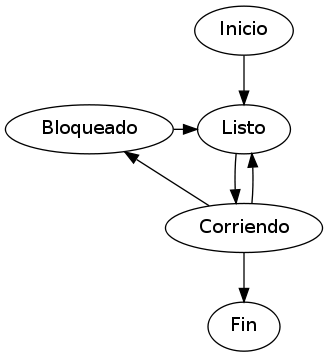
\includegraphics[scale=0.5]{estados.png}
\end{center}
 
En este gráfico de estados podemos apreciar el desalojo de tareas así como 

\subsection{Análisis del algoritmo}

Al realizar varias pruebas pudimos comprobar que a medida que aumentamos el \textit{quantum} haciéndolo proporcional al total de \textit{ticks} de las tareas, el tiempo necesario para que todas finalicen disminuye.
Esto es lo que podemos apreciar en los gráficos siguientes: las tareas duran todas 10 \textit{ticks} y la cantidad de \textit{blocks} aumenta de 0 a 9.

\begin{figure}[H]
\centering
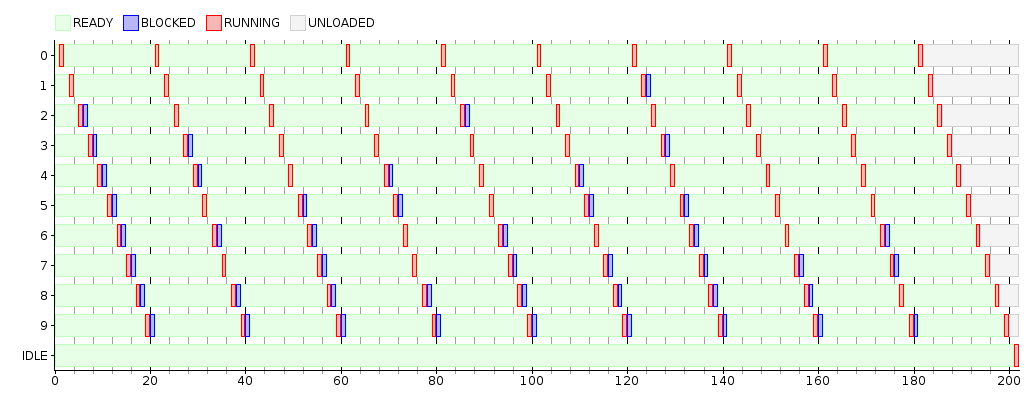
\includegraphics[scale=0.4]{./graficos/out_batch_fijo1.png}
\caption{Algoritmo Round robin con \textit{quantum} 1}
\end{figure}  
 
\begin{figure}[H]
\centering
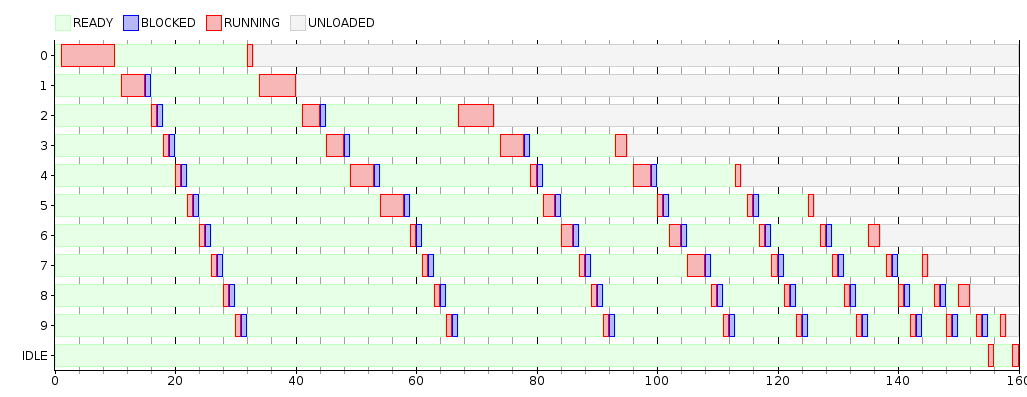
\includegraphics[scale=0.4]{./graficos/out_batch_fijo9.png}
\caption{Algoritmo Round robin con \textit{quantum} 9} 
\end{figure}

Como podemos apreciar en el primer caso las tareas tardan alrededor de 200 \textit{ticks} de reloj en terminar y en el segundo, alrededor de 160. 
	\section{Lottery scheduling}
Lottery scheduling es un algoritmo de planificaci\'on probabilistico para los procesos de un sistema operativo. A cada proceso se les asigna un n\'umero de billetes de loter\'ia, y se elije un boleto al azar para seleccionar el siguiente proceso. La distribución de los billetes no tiene por qu\'e ser uniforme, darle más billetes a un proceso le ofrece una oportunidad mayor de salir seleccionado.

\subsection{Implementaci\'on propuesta}
A la hora de implementar este algoritmo, recurrimos al paper de Waldspurger y Weihl, \textit{Lottery scheduling: Flexible proportional - share resource management} el cual explica los detalles del algoritmo. 

En dicho paper, adem\'as del sistema de tickets se propone un sistema de monedas o \textit{currencies} las cuales respaldan los tickets. El sistema cuenta con una moneda base que respalda una serie de tickets repartidos entre los usuarios que lanzan los procesos. A su vez, cada usuario emite una moneda para respaldar los tickets que reciben sus procesos. Lo mismo sucede con los procesos y sus \textit{threads}. Como en el simulador provisto por la c\'atedra no existen los usuarios ni los \textit{threads}, implementamos \'unicamente el sistema de tickets base.

A continuaci\'on explicaremos los pasos de nuestra implementacion que utiliza los mismos m\'etodos que la vista para Round Robin.

\begin{itemize}
	\item El método \textit{load(pid)} se agrega a nuestro diccionario de tareas el nuevo \textit{pid} y se le da un ticket.
	\item El método \textit{unblock(pid)} se la desmarca como bloqueada.
	\item El método \textit{tick(motivo)} se ejecuta por cada tick del reloj de la máquina el simulador. El parámetro \textbf{motivo} indica lo que ocurrió con la tarea que ocupaba el CPU el ciclo de reloj anterior:
	
	\begin{itemize}
		\item Si el \textbf{motivo} es \textit{exit}: se saca la tarea de nuestro diccionario y se hace un nuevo sorteo.
		\item Si el \textbf{motivo} es \textit{block}: se la demarca como bloqueada y se la compensa con $\frac{quantum}{quantum - f}$ donde \textit{f} es la fracci\'on de \textit{quantum} que utiliz\'o.
		\item Si el \textbf{motivo} es \textit{tick}: si se termina el \textit{quantum} de esa tarea, se la desaloja y se realiza un sorteo. La nueva tarea elegida es puesta a trabajar y se le deja un solo ticket. Si no hay m\'as tareas o est\'an todas bloqueadas, trabaja la \verb|idle_task|.
	\end{itemize}
\end{itemize}

\subsection{Diagrama de estados}
\begin{center}
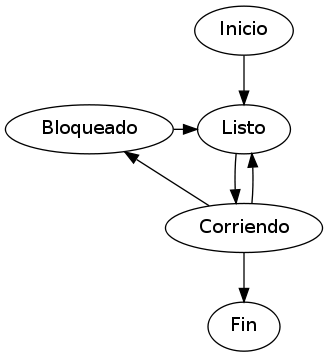
\includegraphics[scale=0.5]{estados.png}
\end{center}

\subsection{An\'alisis del algoritmo}
\begin{figure}[H]
\centering
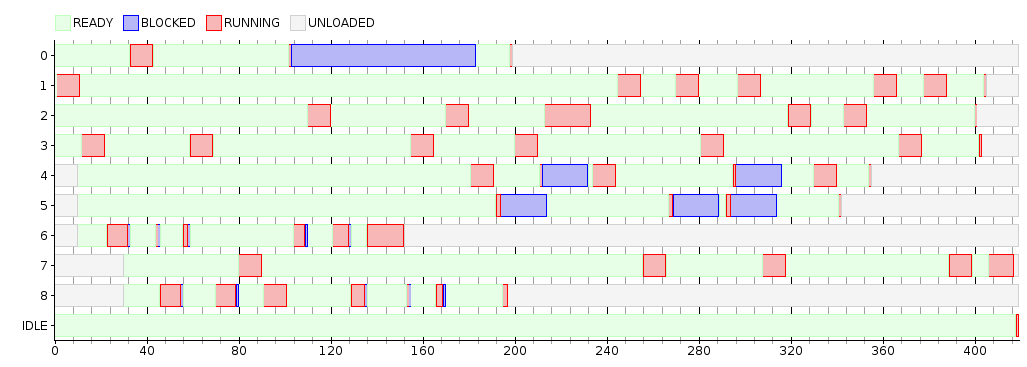
\includegraphics[scale=0.5]{./graficos/out_ej_8.png}
\caption{Lottery - Quantum 10, Semilla 1315772865}
\end{figure} 

\begin{figure}[H]
\centering
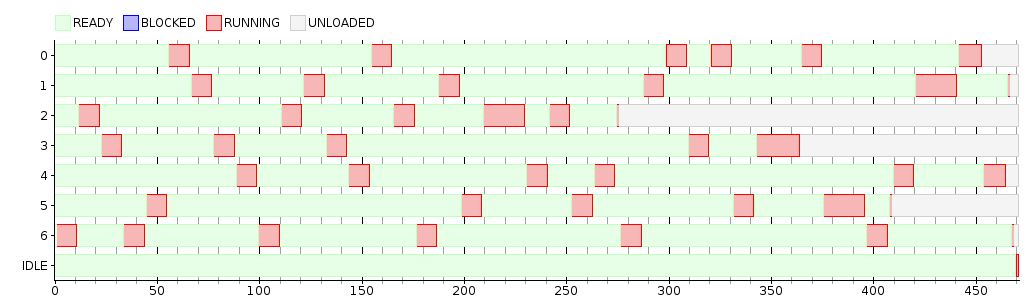
\includegraphics[scale=0.5]{./graficos/out_ej_8_2.png}
\caption{Lottery - Quantum 10, Semilla 1315772865}
\end{figure} 

\begin{figure}[H]
\centering
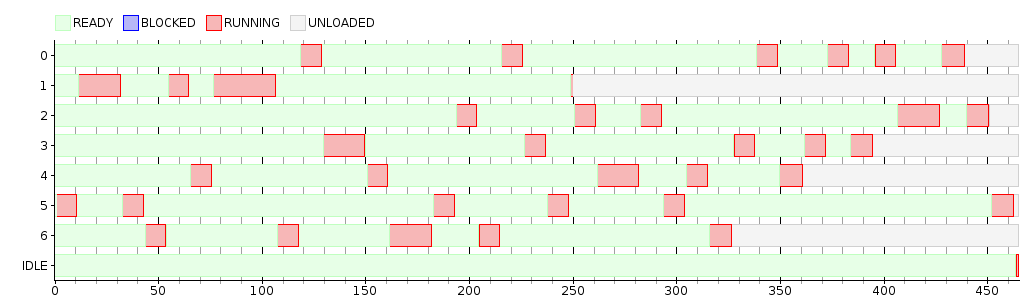
\includegraphics[scale=0.5]{./graficos/out_ej_8_3.png}
\caption{Lottery - Quantum 10, Semilla 1315793579}
\end{figure} 


	%\begin{thebibliography}{9}

\bibitem {} Thomas H. Cormen, Charles E. Leiserson, Ronald L. Rivest, y Clifford Stein. Introduction to Algorithms, Second Edition. MIT Press and McGraw-Hill, 2001.

\bibitem {} Xumari, G.L. Introduction to dynamic programming. Wilwy $\&$ Sons Inc., New York. 1967.

\end{thebibliography}

	%palmitos, champignones a la provenzal 2, panceta y ciruela,
	%provolone 3, queso al oreganato 2, pollo 1
	
	%panceta? anana?

\end{document}